\documentclass{article}

%% PAQUETES

% Paquetes generales
\usepackage[margin=2cm, paperwidth=210mm, paperheight=297mm]{geometry}
\usepackage[spanish]{babel}
\usepackage[utf8]{inputenc}
\usepackage{gensymb}

% Paquetes para estilos
\usepackage{textcomp}
\usepackage{setspace}
\usepackage{colortbl}
\usepackage{color}
\usepackage{color}
\usepackage{upquote}
\usepackage{xcolor}
\usepackage{listings}
\usepackage{caption}
\usepackage[T1]{fontenc}
\usepackage[scaled]{beramono}

% Paquetes extras
\usepackage{amssymb}
\usepackage{float}
\usepackage{graphicx}
\usepackage{url}

%% Fin PAQUETES


% Definición de preferencias para la impresión de código fuente.
%% Colores
\definecolor{gray99}{gray}{.99}
\definecolor{gray95}{gray}{.95}
\definecolor{gray75}{gray}{.75}
\definecolor{gray50}{gray}{.50}
\definecolor{keywords_blue}{rgb}{0.13,0.13,1}
\definecolor{comments_green}{rgb}{0,0.5,0}
\definecolor{strings_red}{rgb}{0.9,0,0}

%% Caja de código
\DeclareCaptionFont{white}{\color{white}}
\DeclareCaptionFont{style_labelfont}{\color{black}\textbf}
\DeclareCaptionFont{style_textfont}{\it\color{black}}
\DeclareCaptionFormat{listing}{\colorbox{gray95}{\parbox{16.78cm}{#1#2#3}}}
\captionsetup[lstlisting]{format=listing,labelfont=style_labelfont,textfont=style_textfont}

\lstset{
	aboveskip = {1.5\baselineskip},
	backgroundcolor = \color{gray99},
	basicstyle = \ttfamily\footnotesize,
	breakatwhitespace = true,   
	breaklines = true,
	captionpos = t,
	columns = fixed,
	commentstyle = \color{comments_green},
	escapeinside = {\%*}{*)}, 
	extendedchars = true,
	frame = lines,
	keywordstyle = \color{keywords_blue}\bfseries,
	language = Oz,                       
	numbers = left,
	numbersep = 5pt,
	numberstyle = \tiny\ttfamily\color{gray50},
	prebreak = \raisebox{0ex}[0ex][0ex]{\ensuremath{\hookleftarrow}},
	rulecolor = \color{gray75},
	showspaces = false,
	showstringspaces = false, 
	showtabs = false,
	stepnumber = 1,
	stringstyle = \color{strings_red},                                    
	tabsize = 2,
	title = \null, % Default value: title=\lstname
	upquote = true,                  
}

%% FIGURAS
\captionsetup[figure]{labelfont=bf,textfont=it}
%% TABLAS
\captionsetup[table]{labelfont=bf,textfont=it}

% COMANDOS

%% Titulo de las cajas de código
\renewcommand{\lstlistingname}{Código}
%% Titulo de las figuras
\renewcommand{\figurename}{Figura}
%% Titulo de las tablas
\renewcommand{\tablename}{Tabla}
%% Referencia a los códigos
\newcommand{\refcode}[1]{\textit{Código \ref{#1}}}
%% Referencia a las imagenes
\newcommand{\refimage}[1]{\textit{Imagen \ref{#1}}}


\begin{document}

% Inserción del título, autores y fecha.
\title{\Large 75.42 Taller de Programación I \\ 
	  \medskip\Huge Informe: Ejercicio N° 4  \\
	  \bigskip\Large\textit{``El código Draka (desencripción por fuerza bruta)''}}
\date{}
\maketitle




% INTRODUCCIÓN
\section{Introducción}
	
	Nuestros agentes han finalmente recuperado el código utilizado por los \textit{Draka} para encriptar y desencriptar sus mensajes. Si bien el código es relativamente simple, no ha sido posible encontrarle vulnerabilidades hasta el momento. Solo se sabe que los textos encriptados son ASCII \cite{ASCII} (códigos de carácter menores a 128) y que las claves solo utilizan dígitos ASCII. Aparentemente, debido a esto, la única opción para recuperar el texto será realizar un ataque de \textit{fuerza bruta} \cite{FB}.
	\par
	Las claves utilizadas son de longitud suficiente como para hacer que un ataque por fuerza bruta con una sola máquina lleve una excesiva cantidad de tiempo. Por lo tanto, se optará por una solución distribuida siguiendo un esquema cliente-servidor: el servidor se encargará de fraccionar el trabajo y los clientes de resolver cada una de estas partes, enviando los resultados al servidor.
	\par
	Detalles mas precisos de la problemática y de las condiciones preestablecidas se pueden encontrar en el enunciado del ejercicio\footnote{Se ha evitado hacer un relevamiento de la totalidad de la información que nos fue conferida, de manera de poder mantener el foco del informe en la forma en que se ha encarado la solución del problema.}.
\bigskip




% CONSIDERACIONES DE DISEÑO
\section{Consideraciones de diseño}

	Para la correcta implementación de la solución fue necesario plantear y establecer cómo se debería comportar el sistema ante ciertas situaciones que no fueron especificadas en el enunciado del problema. A continuación se listan las contemplaciones instauradas:

\begin{itemize}
	\itemsep=3pt \topsep=0pt \partopsep=0pt \parskip=0pt \parsep=0pt

	\item Al producirse una solicitud de trabajo por parte de un cliente, si el servidor le indica que no hay trabajo para asignarle, ambos entes cerraran la conexión que los vinculaba;

	\item El servidor almacenará todas las posibles claves, para una vez finalizada la actividad de todos los clientes, determinar si existe una ambig\"uedad o si es única la clave;

	\item En el envío y en la recepción de datos se considera como fin de mensaje al caractér ``\textit{$\backslash$n}'' establecido por el protocolo.

	\item El programa del lado servidor no finalizará su ejecución hasta cuando y en tanto no se haya introducido ``\textit{q$\backslash$n}'' por la entrada estándar.
\end{itemize}
\medskip




% DISEÑO
\section{Diseño}

	Como se mencionó anteriormente, se optará por una solución distribuida siguiendo un esquema cliente-servidor. De esta manera, poseeremos dos implementaciones independientes una de la otra, pero que trabajaran en conjunto una vez establecida la conexión entre las mismas. Por lo tanto, vamos a tener un programa \textit{servidor} y otro programa \textit{cliente}.
	\par
	En los apartados que siguen pondremos la atención en aquellos aspectos de la implementación de ambos programas que pueden ser relevantes a causa de su complejidad o particularidad. En estos se describen los inconvenientes que presentan y la forma en que fueron resueltos.
\bigskip



% DISEÑO - Cliente
\subsection{Cliente}
	
	Sin duda alguna, este ente del esquema es el menos complejo ya que su tarea se reduce a establecer inicialmente una conexión con el servidor, para luego solicitarle una parte del trabajo a realizar. En el caso de que el servidor le indique que no trabajo disponible, el cliente simplemente finalizará su ejecución. En el otro caso, recibirá el mensaje encriptado y el rango de claves y por fuerza bruta probara cada una de ellas, notificando a través del socket cuales son posibles claves. Finalizadas las pruebas termina su ejecución.
	\bigskip	



% DISEÑO - Servidor
\subsection{Servidor}

	Para el funcionamiento del servidor, se ha propuesto utilizar una lógica muy simple. Esta consiste en tener a la clase \textit{Servidor}, la cual es un hilo de ejecución, esperando por solicitudes de conexión por parte de los clientes. Cuando se produce una situación como la anterior, el mismo servidor se encarga de crear un objeto de la clase \textit{ConexionCliente}. A este objeto se le pasa el file descriptor correspondiente al nuevo socket que mantendrá en contacto al cliente con este último objeto. Este será almacenado en una lista de conexiones existentes, para permitir al servidor saber que conexiones debe cerrar cuando llegue el momento de concluir la ejecución.
	\par
	El objeto de la clase \textit{ConexionCliente} ahora es el único encargado de mantener una comunicación con su par del otro lado del socket. Entre estos se hará el envío de mensajes protocolares los cuales permitiran la asignación de tareas, notificación de posibles claves, entre otras. 
	\par
	Por otro lado, los objetos mencionados en el párrafo anterior son supervisados por la clase \textit{ControladorDeTareas}, la cual es un ente creado por el servidor, y que posee la responsabilidad de, ante una petición, asignar trabajo, de ser posible, al cliente. Además es el que, una vez arrivada una clave, la recibe para almacenarla, permitiendole al servidor posteriormente dar cuenta de ello.
	\bigskip\bigskip




% ESQUEMA DEL DISEÑO
\section{Esquema del diseño}

	A continuación, en la \textit{Figura 1}, se ilustra el diagrama de clases principal, donde se pueden ver las clases que intervienen tanto en el
	servidor como así también en el cliente. Cabe destacar que se han omitido,
	para mayor comprensión, otras clases secundarias pero que hacen a la totalidad del sistema. 
	\bigskip\bigskip\bigskip\bigskip



% REFERENCIAS
\begin{thebibliography}{99}

	\bibitem{ASCII} Código ASCII, \url{http://en.wikipedia.org/wiki/ASCII}
	\bibitem{FB} Ataque por Fuerza Bruta (Brute-force attack), \url{http://en.wikipedia.orig/wiki/Brute-force_attack}
	\end{thebibliography}

\newpage
% Figura 1
\begin{figure}[h]
	\centering
	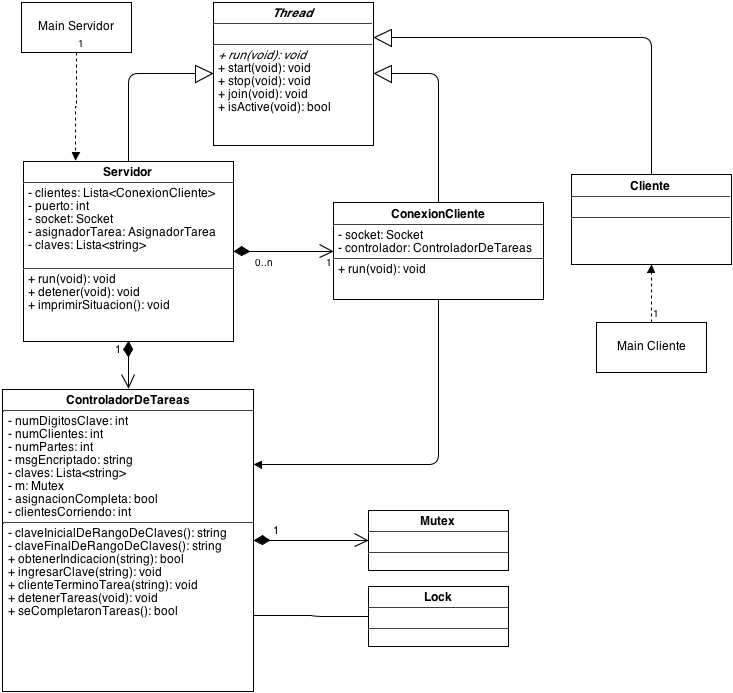
\includegraphics[width=0.968976\textwidth]{images/diagrama_clases.png}
	\medskip
	\caption{Diagrama de clases principales que representan la solución}
\end{figure}
\bigskip



\end{document}
